\chapter{Desenvolvimento}

\section{A Nota Fiscal de Consumidor Eletrônica}

%% FIXME: ReferÊncia http://nfce.encat.org/institucional/o-que-e-nfc-e/
A Nota Fiscal de Consumidor Eletrônica (NFC-e) visa ser uma alternativa eletrônica aos antigos cupons fiscais emitidos em papel. Tal documento segue um modelo nacional de emissão de documento fiscal com validade jurídica garantida pela assinatura digital do emissor.

Com a publicação do Decreto nº 44.785 em 12 de maio de 2014, a NFC-e foi instituída no Estado do Rio de Janeiro a partir do dia seguinte à publicação. Com isso, todos os estabelecimentos comerciais deveriam estar aptos ao uso da NFC-e até o dia 31 de dezembro de 2017.

% FIXME: Ajustar a imagem
% FIXME: Adicionar referencia a imagem
\begin{figure}[h]
    \centering
    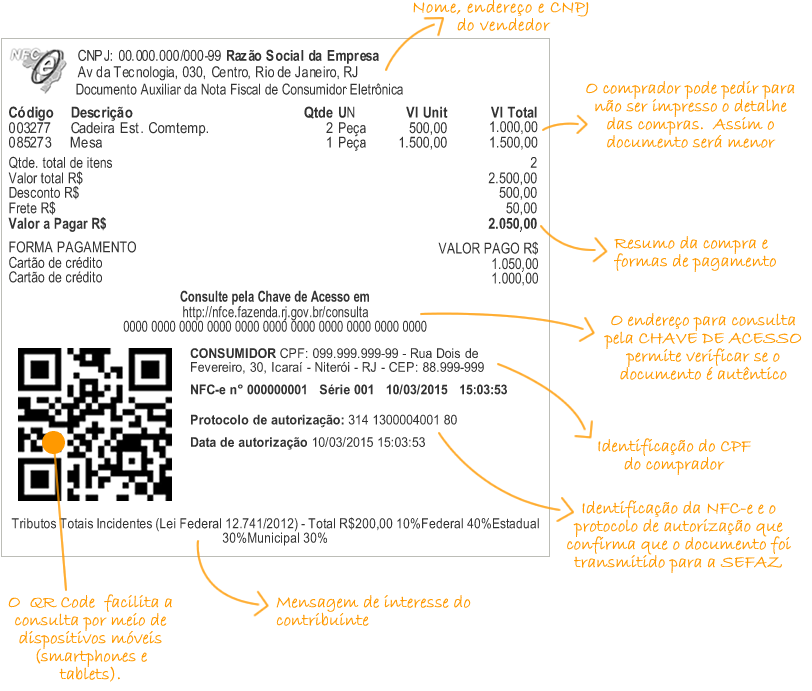
\includegraphics[scale=0.5]{modelo_nota_fiscal}
    \caption{Exemplo de uma NFC-e}
    \label{modeloNfce}
\end{figure}

Na figura \ref{modeloNfce} é possível observar um exemplo de uma NFC-e, com isso, pode se observar a descrição, a quantidade e o preço unitário de cada produto comprado. Além disso, ainda consta a informação do estabelecimento onde a compra foi efetuada como o endereço, o CNPJ e nome do estabelecimento.

Ainda, nesse documento consta uma chave de acesso que é composta por 44 dígitos e um QR Code, de posse desses dados é possível acessar a versão online da respectiva nota, no qual contém as mesmas informações a respeito da compra assim como existe em sua versão física.

% TODO: Adicionar print imagem nota online?

A verificação de autenticidade pode ser efetuada através de um site disponibilizado e mantido por cada Secretaria de Fazenda dos estados que constituem a União. Sendo assim, não é possível verificar a autenticidade de uma NFC-e emitida no estado de São Paulo na plataforma disponibilizada pelo Secretaria de Fazenda do Estado do Rio de Janeiro.

Essa peculiaridade, faz com que a versão desenvolvida descrita nesse projeto, tenha suporte a somente notas emitidas no estado Fluminense. Todavia, a adição do suporte a outros estados é facilitada, pois a inclusão já foi prevista durante o desenvolvimento.

\section{Obtenção das informações}
\label{obtencaoInformacoes}

O usuário pode acessar a versão da online da nota fiscal através de duas formas: a partir de um site específico junto de uma chave de acesso ou pelo site contido no QRCode. Após o usuário solicitar a adição de uma nota fiscal no aplicativo é feita uma simulação de uma dessas formas de acesso resultando em uma requisição ao site da Secretaria de Fazenda.

Independente de que forma foi efetuado o acesso, após o término da solicitação, o usuário é redirecionado para uma página que contém a versão online da nota fiscal. O conteúdo dessa página é analisado e armazenado. A técnica utilizada para a análise desse conteúdo é o Web Scraping.

\subsection{Simulação da solicitação}

Conforme dito anteriormente, independente da forma de acesso à nota, o mesmo conteúdo poderá ser obtido, porém os processos de reprodução dessas formas possuem algumas diferenças entre si.

A solicitação através da chave de acesso é feita de forma a simular o acesso do usuário ao site original, isto é feito com o auxílio da biblioteca Puppeteer para o Node.js é possível reproduzir a navegação em um navegador. Desta forma, o site disponibilizado para consulta das notas é acessado com o auxílio dessa ferramenta, no entanto, para obter o conteúdo da nota é necessário que um código de verificação (código Captcha) também seja inserido para que se possa comprovar que a solicitação está sendo feito por um humano e não por ferramentar automatizadas, logo, esse código é repassado para o usuário do aplicativo para que a requisição possa ser validada.

% FIXME: Melhorar esse trecho.

Caso a nota fiscal já esteja disponível e o código de verificação esteja correto, o conteúdo será disponibilizado, caso contrário, o usuário será notificado que houve um erro durante o cadastro da NFC-e na aplicação.

Já para reprodução com o QRCode, é possível obter o conteúdo diretamente sem a necessidade de inserção de código de verificação, todavia, ainda é necessária a simulação da navegação com o Puppeteer.

Assim como no forma anterior, caso a NFC-e não seja encontrada no sistema da SEFAZ, o usuário também será notificado que a mesma não encontra-se disponível.

Vale destacar que para a adição da NFC-e com o QRCode, é necessário o usuário possua um smartphone com câmera.

Caso qualquer error não previsto durante o processamento da requisição ocorra ou o sistema da SEFAZ esteja inoperante, o usuário também será notificado sobre a impossibilidade da adição com uma mensagem de erro genérica. Tal situação poderá ocorrer independente de que forma foi feita a solicitação.

\subsection{Análise dos dados}

A análise dos dados é feita com o auxílio da ferramenta Cheerio, que é um módulo baseado no jQuery, um framework bastante popular do JavaScript, para utilização com o Node.js. Com o conteúdo da página, é possível obter cada informação individualmente, logo é possível quais produtos foram comprados como o preço unitário e quantidade comprada de cada. Além disso, também é possível armazenar os dados do local da compra como o nome do estabelecimento e o seu endereço. Por fim, dados gerais da compra também podem ser recuperados como a data e a hora em que foi realizada.

A recuperação da informação da página pois o conteúdo é construído com a linguagem HTML e através dos elementos que compõe a página, é possível identificá-los e efetuar a separação da informação.

\section{Armazenamento das informações}
\label{armazenamentoInfo}

% TODO: Modelagem dos dados
% https://medium.com/@gpanassol/como-posso-fazer-modelagem-de-dados-em-mongodb-ea61268ee10b
% https://felipetoscano.com.br/modelando-dados-no-mongodb/
% file:///home/vitor/%C3%81rea%20de%20Trabalho/[NoSQL%20e%20MongoDB%20Users]%20Modelagem%20de%20Dados%20para%20BD%20Orientado%20a%20Documentos.pdf
% https://www.univates.br/bdu/bitstream/10737/1674/1/2017MarcelKober.PDF
% https://www.monografias.ufop.br/bitstream/35400000/1963/6/MONOGRAFIA_An%C3%A1liseProjetosBanco.pdf
Com os dados provenientes da NFC-e já processados, ou seja, analisados e separados, esse conteúdo resultante é armazenado em um banco de dados para que a informação seja disponibilizada posteriormente para consultas a partir da aplicação.

Esse conteúdo é armazendao em um banco de dados e o tipo utilizado pela aplicação é o MongoDB, que é um banco de dados não-relacional com os dados sendo armazenados em formato de documento. Como a aplicação está sendo feita em JavaScript, foi optado em utilizar essa banco devido a conveniência resultante do uso junto ao Json.

Além disso, esse tipo de banco é altamente escalável, isto é, caso seja necessário mais espaço para o armazenamento dos dados, o conteúdo pode ser distribuído em diversas máquinas sem afetar o desempenho geral da aplicação.

\subsection{Justificativa do uso de Armazenamento Remoto e os Dados compartilhados}

Os dados provenientes do processamento das notas fiscais poderiam ser armazenados nos celulares dos usuários do aplicativo, o que resultaria no consumo de espaço de armazenamento que é também compartilhado com outros aplicativo e o sistema operacional do aparelho móvel. Embora seja uma alternativa viável para o cliente, e possivelmente rápida, uma vez que a recuperação não sofrerá latência de rede, a longo prazo talvez não seja considerada muito atrativa. A justificativa dessa afirmação é o fato de que para cada nota adicionada uma parcela do armazenamento é consumida, ademais, não existe uma rotina de limpeza dos dados mais antigos.

Apesar da implementação dessa rotina ser simples, restringiria uma possível melhoria ao produto, por exemplo, a disponibilização da série histórica de preços dos produtos a longo prazo.

Um outro ponto que pode ser destacado, é que com os dados concentrados no dispositivo de um indivíduo, os mesmos estão propensos a exclusão, que pode ser causada por diversas situações, por exemplo, a eliminação decorrente da remoção do aplicativo, a formatação do aparelho devido a restauração ao modo de fábrica ou até mesmo uma pane no aparelho em certos casos.

Após a observação dos pontos acima, a utilização de uma solução que envolva o armazenamento da informação em um meio externo torna-se viável, pois a segurança da informação é melhor garantida, uma vez que a cópia de segurança é garantida do lado do servidor desonerando o cliente dessa responsabilidade.

Uma vantagem garantida com ao preservar os dados dessa forma, é que uma base maior pode ser criada pois as notas de todos os usuários poderão estar guardadas em único local, o que acarreta em um compartilhamento de informação e a criação de uma base de dados colaborativa, aonde um usuário A adiciona sua NFC-e e os dados dos produtos estarão disponíveis para um usuário B, e caso esse último quisesse saber o custo de um produto comprado pelo usuário A, poderia consultá-lo por meio do aplicativo sem a necessidade de ir ao mercado utilizado pelo usuário A.

Vale destacar que, apesar da utilização de uma base compartilhada, não há como um usuário ter acesso ao valor gasto em uma compra de outro usuário, uma vez que as notas são adicionadas sem a necessidade de um cadastro e somente é possível obter a informação de produtos, e não de uma compra como um todo.

% TODO: Melhorar seção
\section{Disponibilização dos dados}

% Dependnecia de internet vs offilien
% Contraatacar com o processamento

% Processamento no proprio aparelho
% Usar do processador / bateria/internet de qualidade /

Os dados são disponibilizados com o auxílio do servidor principal da aplicação no qual possui uma conexão com o servidor em que se encontra o banco de dados.

% FIXME: Deve-se referenciar o Framework?
Através do Framework Express é possível criar de uma forma flexível uma API, que permite a comunicação com outras aplicações. Com isso, é disponibilizada uma URL que permite a consulta dos produtos salvos na base de dados.

A consulta é feita através do nome do produto, e esse nome pode estar acentuado corretamento, erroneamente ou até mesmo sem acentos, que os mesmos dados serão retornados.

Os dados retornados contém o nome do produto da forma que consta na nota fiscal, o nome do estabelecimento no qual a compra foi efetuada e a data e a hora da compra. Para cada produto compatível com a consulta, é retornado o último registro salvo para cada estabelecimento para que o usuário sempre possa ter o preço mais recente.

Vale ressaltar que é possível refinar a cidade em que a consulta deverá ser feita, assim como retornar os registros de todas as cidades disponíveis.

\subsection{Ausência de padronização nos nomes}

Um problema que pode ser observado a partir de uma simples consulta com o aplicativo é a ausência de padronização nos nomes dos produtos, haja vista que cada mercado cadastra em seu banco de dados as informações referentes aos produtos a seu bel-prazer. Como também, devido a espaço limitado nas notas fiscais impressas, faz com que ocorra uma abreviação nos produtos.

Uma alternativa aos nomes que poderia ser utilizada, poderia ser através do código de barras presente em cada produto, por outro lado, para aqueles produtos que são vendidos por peso, não há uma uniformidade no código desses produtos, ficando a critério de cada estabelecimento definir um código.

Visto esses problemas descritos, uma solução híbrida pode ser utilizada, isto é, dado um nome de um produto, com auxílio de serviços de terceiros, é possível recuperar o código de barras para o produto pesquisado, com isso, poderia efetuar a busca tanto pelo nome quanto pelo código de barras. Essa solução é sugerida como uma melhoria futura para a aplicação.

\section{Hospedagem}

Conforme descrito nas secções \ref{obtencaoInformacoes} e \ref{armazenamentoInfo}, um servidor torna-se necessário tanto para o processamento e disponibilização dos dados quanto para o armazenamento dos mesmos. Com isso um serviço de hospedagem faz-se necessário para ambos os casos.

\subsection{Backend}

Como todo processamento dos dados é feito em meio externo ao telefone móvel do usuário, logo, a utilização de um servidor é necessária e com isso será necessário a utilização de máquinas para poder executar o código desenvolvido para esse propósito. Um computador pessoal de baixo custo atende esse requisito, no entanto, a medida que o uso do aplicativo tornar-se mais frequente e a base de cliente for aumentando, uma máquina com mais recursos será imprescindível.

O uso de uma máquina física para esses propósitos é uma solução viável, no entanto, existem serviços que fornecem recursos de hospedagem a custo acessível e caso elegível, até mesmo, gratuito.

Uma das principais vantagens do uso de serviços de hospedagem é que o serviço não será interrompido caso haja queda de energia ou até mesmo ficar sem conexão com a internet.

Um dos serviços mais populares que oferecem tais recursos de hospedagem é o Heroku, que fornece desde uma máquina simples gratuita até serviços mais robustos focados para o uso de alto fluxo de dados como ocorre em grandes corporações.

Durante o desenvolvimento os primeiros meses de desenvolvimento, foi feito o uso da plano gratuito para testes, no entanto caso não houvesse nenhuma iteração com a API desenvolvida durante um período de 30 minutos, a mesma ficaria inativa. Diante desse fato, a solicitação de adição de notas tornava-se mais lenta pois além do tempo de processamento dos dados, o tempo de inicialização aumentava a latência em que a resposta era retornada ao usuário. Todavia, a iteração ainda poderia ser feita normalmente.

% TODO: Add ref https://education.github.com/pack
A empresa GitHub, que permite que desenvolvedores e empresas armazenem e divulguem seus códigos, possui um programa para estudantes que permite que os mesmos acessem e usufruem de recursos pagos sem gerar nenhum ônus. Esse programa é conhecido como GitHub Student Developer Pack que é feito em parceria com outras empresas do ramo da tecnologia.

O Heroku é um serviço que está incluso nessa parceria fornecendo uma máquina paga com muitos recursos sem nenhum custo ao estudante participante desse programa por um período limitante. Como o autor é elegível, o uso dessa máquina paga está sendo feito para os testes simulando o uso real de um servidor que pode ser utilizado em produção, isto é, recebendo altas cargas de requisições.

Outras empresas que poderiam ser utilizadas seriam a DigitalOcean, Locaweb, Hostgator e quaisquer outras com recursos semelhantes.

\subsection{Banco de Dados}

% TODO: Adicionar sugestões
% Acho que sim, voce pode mencionar os benefícios que voce teve por ser estudante, no momento do desenvolvimento do trabalho.
% E tambem mostrar alternativas para qunado nao é estudante.

\section{Desenvolvimento do aplicativo}\label{desenvApp}

O desenvolvimento do aplicativo é feito utilizando uma tecnologia de desenvolvimento multiplataforma com código nativo, para isso foi utilizado o React Native. Com isso, é possível desenvolver um único aplicativo e publicar para as duas plataformas mais populares, isto é, o IOS e o Android.

Com isso foi feito o desenvolvimento de único aplicativo que pode ser utilizado nas duas plataformas mencionadas acima. Sendo feito dessa forma, houve uma otimização no tempo de desenvolvimento.

% FIXME: Referenciar o ranking?
A justificativa para a escolha do uso do React Native, primeiramente é pelo fato de permitir um desenvolvimento multiplataforma com código nativo, em acréscimo, estava melhor colocado no ranking elaborado pelo StackOverflow, \textcolor{red}{\textbf{[presente na seção {TEMP} Devo referenciar o ranking?]}} quando comparado com seus concorrentes diretos. Além disso, caso futuramente seja disponibilizado as mesmas funcionalidades presentes no aplicativo para um website, isso poderá ser feito sem muitas complicações, sendo necessária poucas alterações.

\subsection{Expo}

%% FIXME:  Add ref https://docs.expo.io/versions/v36.0.0/; https://docs.expo.io/versions/latest/sdk/overview/
O Expo é um Framework e uma plataforma para aplicações de React. Com isso, acaba por ser um conjunto de ferramentas e serviços criadas em torno do React Native e das plataformas nativas que permite ao programador, desenvolver e distribuir sua aplicação entre os sistemas facilmente, a partir do mesmo código desenvolvido em JavaScript.

Além disso, o Expo proporciona uma abstração dos recursos de aparelhos móveis sem a necessidade de implementação de código nativo. Os recursos são tais como os contatos, a câmera, acesso ao GPS e dentre outros. Com isso, é possível recuperar a informação proveniente desses através do próprio código em JavaScript.

Com isso, foi optado em utilizar essa ferramenta de forma a acelerar o desenvolvimento do aplicativo. Como também é necessário o acesso a câmera para a leitura de QRCodes, tal ferramenta tornou-se indispensável, pois, por ser uma abstração de código nativo, é possível disponibilizar essa funcionalidade para ambas as plataformas sem complicações.

% Explicar a facilidade que o Expo proporciona
% Port para as aplicações

\subsection{Estilização}

De forma a acelerar o tempo de desenvolvimento do aplicativo, algumas ferramentas foram utilizadas para a estilização do aplicativo. Tais ferramentas são um conjunto de componentes prontos, isto é, já estilizados, bastando somente efetuar a adaptação para o projeto como o posicionamento e o tamanho.

Desses recursos, foram utilizados dois pacotes de estilos, o NativeBase e o React Native Paper. Ambos, fornecem estilos semelhantes aos nativos disponíveis em cada plataforma.

% NativeBase
% Native Paper

% Falar aqui dos templates usados com o React Native
% Vantagem de manter o estilo nativo para o Android e o IOS